\chapter{Methodology}\label{methodology}

\begin{figure}[t]
    \centering
    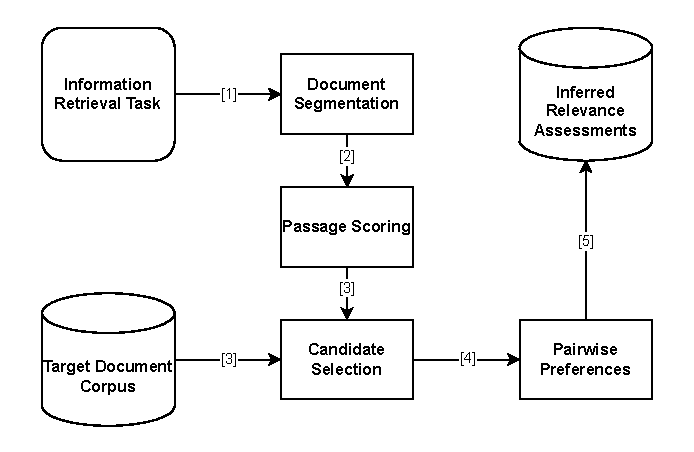
\includegraphics[width=\textwidth]{./graphics/drawio/transfer_pipeline.pdf}
    \caption{Overview of the transfer pipeline and its individual steps to transfer exisiting relevance judgments into another document corpus.}
    \label{fig:transfer-pipeline}
\end{figure}

In this Chapter, I present the individual steps of the developed pipeline used for relevance transfer. The process begins with an information retrieval task consisting of a document corpus, a set of queries, and corresponding relevance judgments (Figure~\ref{fig:datasets}). The goal of the pipeline is to transfer the information of existing relevance judgments from a retrieval task to a target document corpus, thereby generating new relevance judgments. A simplified overview of the process is shown in Figure \ref{fig:transfer-pipeline}, which will now be explained in detail.
\\\\
The first step in the transfer pipeline involves selecting and segmenting documents from the retrieval task's document corpus. Only documents that contain at least one relevance judgment are selected, as those without any judgment do not provide useful information for the transfer process. Once selected, these documents are segmented into passages. This segmentation is done because relevant information related to an information need is typically concentrated in specific sections rather than spread across the entire document. By breaking documents into passages, the focus remains on the most relevant content. Additionally, since later stages of the pipeline rely on large language models, limiting the size of processed text through segmentation helps prevent potential issues when handling long documents with transformer models.
\\\\
The second step focuses on identifying the most relevant passages within each selected document. Therefore, the relevance of each passage is determined in respect to the query of its document's relevance judgment. To achieve this, each passage is treated as an independent query and submitted to the source document corpus. The resulting document ranking is then used to compute various evaluation metrics, which are assigned as passage scores. These scores are later used for selecting candidate documents from the target document corpus and identifying source passages for pairwise preference comparisons.
\\\\
The third step is the selection of candidate documents from the target document corpus. For each query in a retrieval task, a set of documents is chosen to receive new relevance judgments. This selection is performed using different strategies with the aim to identify documents most likely to be relevant. Each selected target document is then also segmented into passages and each passage is paired with relevant passages from the source dataset, identified in the previous passage scoring step. These candidates serve as input for the pairwise inference process in the last step.
\\\\
At this stage, the transfer pipeline has identified, for each query, a set of target documents along with a corresponding set of relevant passages from the source dataset. The final step is inferring new relevance judgments for the target documents. Therefore, each query is processed alongside a target passage and a source passage using a pairwise ranking model to determine whether the target passage is as relevant for the query as the source passage.\linebreak Finally, a judgment for the entire target document is created by aggregating all of its inferred passage scores.

% ========
% Datasets
% ========
\section{Datasets}\label{datasets}

\begin{table}[t]
    \centering
    \setcitestyle{numbers}
    \footnotesize
    \caption{Source corpora and their retrieval tasks from which query relevance judgments (\texttt{qrels}) were transferred to the target document corpus \texttt{ClueWeb22/b}.}
    \label{tab:datasets}
    \begin{tabular}{cccrrc}
        \toprule
        \multicolumn{2}{c}{\textbf{Corpus}} & \multicolumn{4}{c}{\textbf{ Associated Retrieval Task}} \\
        \cmidrule(lr){1-2} \cmidrule(lr){3-6}
        Name & documents  & Name & Queries &\texttt{qrels} & Labels \\
        \toprule
        
        Args.me~\cite{ajjour:2019} & 0.4~m & Touché 2020 Task 1~\cite{bondarenko:2020} & 49 & $2\,298$ & 3 \\
        \midrule

        \multirow{3}{*}{Disks4+5~\cite{voorhees:1996}} & \multirow{3}{*}{0.5~m} & Robust04~\cite{voorhees:2004} & 250 & $311\,410$ & 3 \\
        & & TREC-7~\cite{voorhees:1998} & 50 & $80\,345$ & 2 \\
        & & TREC-8~\cite{voorhees:1999} & 50 & $86\,830$ & 2 \\
        \midrule

        \multirow{2}{*}{MS MARCO Passage~\cite{bajaj:2016}} & \multirow{2}{*}{8.8~m} & TREC 2019 DL Track~\cite{craswell:2019} & 43 & $9\,260$ & 4 \\
        & & TREC 2020 DL Track~\cite{craswell:2020} & 54 & $11\,386$ & 4 \\
        
        \bottomrule
    \end{tabular}
\end{table}

\begin{figure}[t]
    \centering
    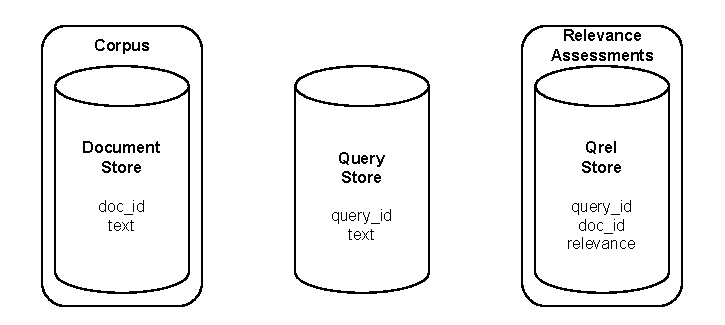
\includegraphics[width=\textwidth]{./graphics/drawio/datasets.pdf}
    \caption{Simplified structure of a dataset from \texttt{ir\_datasets}, comprising a set of documents, queries, and relevance judgments, along with their attributes.}
    \label{fig:datasets}
\end{figure}

Before the actual processing can begin, it is necessary to determine the source and target of the relevance transfer. This involves selecting datasets, along with their associated information retrieval tasks, as the foundation for transferring relevance judgments to a target document corpus.
\\\\
To simplify data handling, I used \texttt{ir\_datasets}~\cite{macavaney:2021}, a Python package that provides access to numerous information retrieval datasets. As illustrated in Figure~\ref{fig:datasets}, each dataset consists of a document corpus, a query store, and a set of query relevance judgments for the queries and documents.
\\\\\\
A key advantage of \texttt{ir\_datasets} is its standardized interface\footnote{\scriptsize https://ir-datasets.com/python.html}, which enables uniform access to different datasets. Through built-in iterators, the package facilitates structured access to corpora, queries, and relevance judgments, allowing the transfer pipeline to handle diverse datasets efficiently.
\\\\
The corpora and associated information retrieval tasks used in this thesis are listed in Table~\ref{tab:datasets}. The source datasets were selected based on their widespread use in information retrieval research and their varying sizes. \texttt{Args.me} and \texttt{Disks4+5} are relatively small corpora, whereas \texttt{MS MARCO Passage} is significantly larger. Additionally, the number of existing relevance judgments in these datasets varies considerably. \texttt{Args.me} contains approximately $2\,300$ judgments, while the retrieval tasks associated with \texttt{MS MARCO} have several thousand. In contrast, the tasks associated with \texttt{Disks4+5} extend far beyond this, with one exceeding $300\,000$ judgments. Notably, the \texttt{MS MARCO} dataset is already preprocessed and provided as passages, unlike the other datasets. This is a significant difference, as the relevance judgments are already at passage level, eliminating the need for further segmentation of the documents. This diversity in dataset size and relevance judgment density provides a robust test for the transfer process under different conditions.
\\\\
The selected datasets serve as the starting point of the pipeline, while the final target corpus for relevance transfer is \texttt{ClueWeb22/b}. This dataset was chosen because it is the newest ClueWeb corpus in the \texttt{Lemur Project}\footnote{\scriptsize https://lemurproject.org}. With over 1.0~billion documents, \texttt{ClueWeb22/b} is significantly large, but due to its recent release, it currently has a low number of relevance judgments. The objective of the transfer process is to enrich \texttt{ClueWeb22/b} by leveraging the existing relevance judgments from the source datasets, thereby enhancing its use cases for information retrieval research.
\pagebreak


% =====================
% Document Segmentation
% =====================
\section{Document Segmentation}\label{document-segmentation}

\begin{figure}[t]
    \centering
    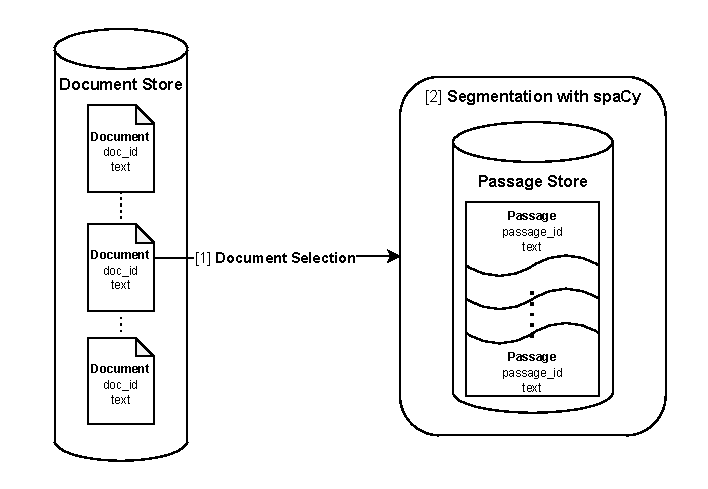
\includegraphics[width=\textwidth]{./graphics/drawio/document_segmentation.pdf}
    \caption{Visualization of the document segmentation step in the transfer pipeline. First, a subset of documents is selected from the source document store. Then, the selected documents are segmented using \texttt{spaCy}.}
    \label{fig:document-segmentation}
\end{figure}

With the selection of the source datasets and the target document corpus \mbox{completed}, the actual processing of the transfer pipeline can begin. To \mbox{provide} a clearer understanding of the individual steps involved, the following explanations will use one source dataset from Table~\ref{tab:datasets} as an illustrative example. The described steps apply uniformly across all corpora and retrieval tasks.
\\\\
The first step involves selecting and segmenting documents from the source dataset into passages, as illustrated in Figure~\ref{fig:document-segmentation}. The primary objective of the pipeline is to transfer the relevance judgments from the source retrieval tasks to the target corpus. This transfer starts by identifying the relevant documents in the source corpus based on the existing relevance judgments for each query in the retrieval task. These documents serve as the foundation for the later pairwise preference step, where they are compared with documents from the target corpus. To reduce computational overhead, only a subset of documents from the source dataset is selected. As demonstrated by \mbox{\cite{gienapp:2022}}, the number of pairwise preferences can be reduced through sampling without significantly impacting effectiveness. Consequently, the pipeline will utilize a limited set of comparison documents rather than all possible documents, minimizing the computational cost. Once the relevant documents have been selected, they are segmented into passages. This segmentation is essential because relevant information related to a query is often confined to specific sections rather than the entire document. By processing documents at the passage level, the pipeline can focus on the most relevant parts while filtering out less relevant parts of a document. Additionally, the subsequent steps of the pipeline involve processing text with transformer models, which have a maximum input length they can handle. Segmenting documents into smaller passages ensures compliance with these constraint, thereby enabling the models to operate effectively \cite{levy:2024}.

% Document Selection
\subsection{Document Selection}\label{document-selection}

Instead of using the entire document corpus for relevance transfer, only a representative selection of documents is used, step one of Figure~\ref{fig:document-segmentation}. First, all documents without relevance judgments in the retrieval task can be ignored since they contain no useful information for the relevance transfer. Therefore, only judged documents are considered for selection. A document is considered judged if it has at least one relevance judgment in the \texttt{qrel store}. These judged documents, along with their relevance judgments for one or multiple queries of the retrieval task, can be used to transfer information, as their relevance has already been determined.
\\\\
As shown in Table~\ref{tab:datasets}, each retrieval task uses different relevance labels to indicate the relevance of a document to a given query. Some datasets apply binary labels, distinguishing simply between relevant and non-relevant documents, while others utilize a Likert scale with multiple relevance levels to represent varying degrees of relevance. In this thesis, no distinction is made between different levels of non-relevance. For instance, \glqq not relevant\grqq{} \mbox{(\texttt{label = 0})} and \glqq strongly not relevant\grqq{} (\texttt{label < 0}) are treated equally. This standardization was applied because finer distinctions between non-relevant documents are not considered necessary for the pipeline, as many TREC evaluation implementations and metrics, such as \texttt{nDCG}, ignore negative labels by mapping them to zero by default \cite{gienapp:2020}.
\\\\\\\\\\
At this stage, all documents with at least one relevance judgment for any query of the retrieval task have been identified. Some retrieval tasks, such as \texttt{Robust04} with over 300,000 relevance judgments, contain a large number of judgments per query. As mentioned above, only a representative subset of judged documents can be used for relevance transfer for each query. To manage this, the number of judged documents in the transfer process is limited. For each query, a maximum of 50 relevance judgments per relevance label of the retrieval task, referred to as a query-label combination, is selected.

% Segmentation with spaCy
\subsection{Segmentation with spaCy}\label{segmentation-with-spacy}

Now that the documents used for relevance transfer have been selected, they are segmented into passages. This segmentation is performed to focus only on the most relevant parts of a document rather than the entire text and to ensure proper processing of text snippets through large language models later. To achieve accurate segmentation with correct sentence separation, the GitHub repository \texttt{grill-lab/trec-cast-tools}\footnote{\scriptsize https://github.com/grill-lab/trec-cast-tools} was utilized. The repository provides a collection of scripts designed to process the TREC CAsT Track 2022~\cite{owoicho:2022}. Among its features is the ability to process a document collection and generate passage splits.
\\\\
\texttt{trec-cast-tools} leverages \texttt{spaCy}\footnote{\scriptsize https://spacy.io}, a powerful natural language processing library in Python. \texttt{spaCy} offers various features such as: tokenization, part-of-speech tagging, named entity recognition, lemmatization, and many more. It also provides functionality for sentence segmentation, which is used by \texttt{trec-cast-tools}. First, the documents are processed by \texttt{spaCy}, splitting the texts into sentences. Then, \texttt{trec-cast-tools} concatenates these sentences into passages, with each passage limited to a maximum length of 250 words. After processing all the selected documents from the source corpus, they are now stored as uniquely identifiable passages, ensuring traceability throughout the transfer pipeline. These passages are saved in the \texttt{passage store}, as shown in the second step of Figure~\ref{fig:document-segmentation}.
\\\\
When a document is judged relevant to a query, the relevant information is often scattered throughout the text. Therefore, the next step in the transfer pipeline is to identify the most relevant passages within each document. This step optimizes the subsequent candidate selection process and improves the effectiveness of the pairwise preference evaluation by ensuring that highly relevant passages from the source corpus are used for comparison.
\pagebreak


% ===============
% Passage Scoring
% ===============
\section{Passage Scoring}\label{passage-scoring}

\begin{figure}[t]
    \centering
    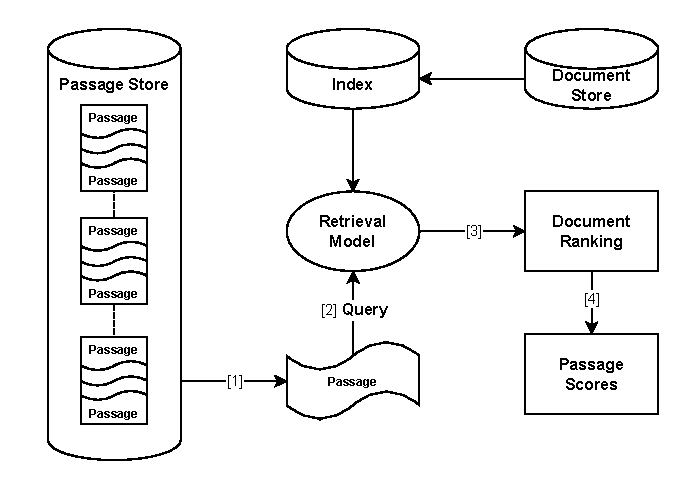
\includegraphics[width=\textwidth]{./graphics/drawio/passage_scoring.pdf}
    \caption{Overview of the passage scoring process, where each passage is submitted as an independent query to its source document corpus, and scores are assigned based on the retrieved document ranking.}
    \label{fig:passage-scoring}
\end{figure}

As selected in Section \ref{document-selection}, each query-label combination of a retrieval task has an associated set of relevance judgments along with their corresponding documents. To determine which passages of a document are most relevant and best reflect the label of its relevance judgment, a ranking of the individual passages is performed in this step. To rank all passages of the selected documents, the following procedure is applied to all passages. First, each passage of a document is treated as an independent query, as shown in step one and two of Figure~\ref{fig:passage-scoring}. This query is then used to retrieve a document ranking from its original source \texttt{document store}, as shown in step three of \mbox{Figure~\ref{fig:passage-scoring}}. Based on the retrieved document ranking for the submitted passage, the relevance of the passage is determined by computing its \texttt{precision@10} and \texttt{nDCG@10} scores, step four of Figure~\ref{fig:passage-scoring}. These metrics were chosen because they are widely used in information retrieval research. In contrast to \texttt{precision}, \texttt{nDCG} provides a more fine-grained evaluation by considering relevance labels of the retrieved documents, whereas \texttt{precision} only accounts for binary relevance.
\\\\
\textbf{Precision} is the fraction of retrieved documents that are relevant to an information need. In this context, the information need corresponds to the original query associated with the relevance judgment of the document to which a passage belongs. A retrieved document is considered relevant if it has been judged as such in the relevance judgments for that query. To simplify the scoring process, the evaluation is restricted to the top 10 retrieved documents. The resulting \texttt{precision@10} score is then assigned as the passage's score, representing its relevance to the query of the document's original relevance judgment.
\\\\
\textbf{Normalized Discounted Cumulative Gain} (\texttt{nDCG}) is another metric commonly used in information retrieval to evaluate the quality of a retrieved document ranking. Similar to \texttt{precision}, the query associated with the relevance judgment of the document to which a passage belongs is used to determine the relevance labels of the retrieved documents. Cumulative Gain (\texttt{CG}) represents the sum of all relevance labels for the retrieved document ranking. Unlike \texttt{precision}, \texttt{CG} takes into account the label values rather than simply differentiating between relevant and non-relevant labels. This provides greater granularity in retrieval tasks with more than two relevance levels, allowing for more nuanced scoring of document passages. The advanced Discounted Cumulative Gain (\texttt{DCG}) further refines this evaluation by introducing a positional factor to the ranking, assigning higher weight to relevant results that appear earlier in the ranking. The final \texttt{nDCG} score is calculated by normalizing the \texttt{DCG} score with the Ideal DCG (\texttt{IDCG}), which represents the optimal theoretical document ranking for the query. As with \texttt{precision}, the evaluation is limited to the first 10 documents by only computing \texttt{nDCG@10}.
\\\\
The idea behind ranking a document's passages is that passages containing a high density of relevant information to an information need (i.e., the original query of a relevance judgment) are more likely to retrieve relevant documents and therefore achieve higher \texttt{precision@10} and \texttt{nDCG@10} scores. Conversely, passages with minimal or no relevant information will lead to lower scores due to fewer retrieved relevant documents.
\\\\
At this stage of the pipeline, the individual passages of the selected documents have been scored. These scores will serve as the foundation for the subsequent steps in identifying candidate documents from the target corpus. The selected candidates will receive newly inferred relevance judgments at the end of the pipeline. Additionally, these scores will help determine the most relevant passages from the source document corpus, which will be used in pairwise preference comparisons alongside the selected target candidates.


% ====================
% Candidate Retreiaval
% ====================
\section{Candidate Selection}\label{candidate-selection}

\begin{figure}[t]
    \centering
    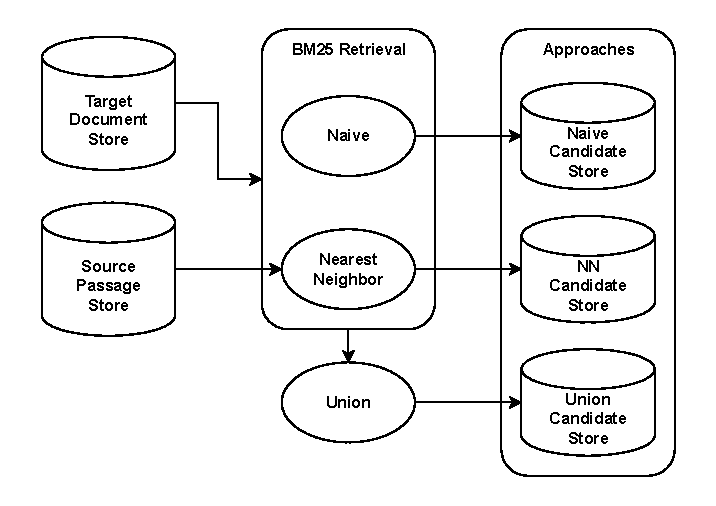
\includegraphics[width=\textwidth]{./graphics/drawio/candidate_selection.pdf}
    \caption{Overview of the three candidate retrieval approaches for selecting documents from the target corpus. The selected candidates will receive new relevance labels inferred at the end of the pipeline.}
\end{figure}

The next step in the transfer pipeline is selecting candidates for pairwise preference inference. This step consists of two parts. First, for each query in a retrieval task, documents from the target corpus are selected. New relevance judgments will be created for these queries and their selected documents. The second part involves choosing passages from the source corpus for each query. These passages will be used in pairwise preference comparison to determine whether a document from the target corpus is relevant to a given query.

% Document Retrieval from Target Dataset
\subsection{Document Retrieval from Target Dataset}\label{document-retrieval-from-target-dataset}

For each query in the retrieval task from the source dataset, a set of documents from the target corpus must be selected for which new relevance judgments will be inferred. The goal is to identify documents that are most likely relevant to a query. By pre-selecting potentially relevant documents, the number of identified relevant documents at the end of the pipeline should be increased.
\\\\
To achieve this, all three tested approaches for selecting target documents begin with \texttt{BM25} retrieval as a pre-selection method. By submitting texts or passages, that are already identified as relevant for a query, against the target document store, a ranking of target documents is retrieved. The highest-ranked documents are most likely to be relevant to the query and therefore qualify for relevance inference. A fine-grained classification of relevance is performed later through the actual pairwise preference inference. \texttt{BM25} retrieval was chosen for its fast retrieval and because only an initial rough assessment is required.
\\\\
\textbf{Naive} The first approach, termed \texttt{naive}, submits each original query text from a retrieval task to the target corpus to retrieve potentially relevant documents. From the resulting document ranking, the top 1000 documents are selected as candidates. Unfortunately, some queries may be ambiguous, leading to multiple possible interpretations. For example, the query \glqq Apple\grqq{} could refer to either the technology company or the fruit. To address such ambiguities, the query narrative is also submitted as an independent query. A query narrative is a brief text that provides additional context, clarifying the search intent and specifying a query's focus. This retrieves another 1000 documents via \texttt{BM25} ranking. After filtering out duplicates between the two sets, up to 2000 unique documents per query are selected.
\\\\
\textbf{Nearest Neighbor} The second approach, \texttt{nearest neighbor}, is based on the relevant passages identified in Section~\ref{passage-scoring}. In this strategy, the top-scoring passages for each query are submitted as queries to the target corpus. For each passage, the top 20 documents in the retrieved document ranking are selected as candidates for the corresponding query. As a result, each passage can contribute up to 20 unique documents to the candidate set. Additionally, several variations of the \texttt{nearest neighbor} approach were tested to determine the most effective candidate selection strategy. First, the number of top passages per query from the source dataset was limited. Three variations were evaluated: one using the top 10 passages, another using the top 50, and a third using the top 100 passages. This limitation significantly reduces the number of potential candidates, as a single query can have an exceedingly large number of relevant passages. The second variation is restricting the selection to one passage per source document. For example, if the top 10 passages for a query contained multiple passages from the same document, only the best-scoring passage is used for retrieving. The intention behind this restriction is to ensure greater diversity in the retrieved candidates. Conversely, an alternative approach permits multiple passages from the same document. This variation was tested to assess the impact of passage diversity on retrieval effectiveness.
\\\\
\textbf{Union Approach} The third approach, called \texttt{union}, combines the \texttt{naive} and \texttt{nearest neighbor} approaches into a single candidate set for each query. This combination is intended to enhance the recall of retrieved relevant documents by including a broader set of potentially relevant documents. However, the increased number of documents will reduce precision by allowing more irrelevant documents to be included, thereby increasing the workload for pairwise preference evaluations in later stages. A detailed evaluation of the various candidate retrieval approaches is done in Section~\ref{eval-candidate-selection}.

% Postprocessing of Selected Target Documents
\subsection{Postprocessing of Selected Target Documents}\label{postprocessing-of-selected-target-documents}

As described in Section~\ref{segmentation-with-spacy}, selected documents from the target corpus are segmented into passages for later processing. Since pairwise preferences will be applied at passage level, documents from both the source and target datasets have to be divided into passages. Therefore, the selected candidate documents are processed with \texttt{trec-cast-tools} as outlined before. First, \texttt{spaCy} is employed for segmenting the chosen target documents into sentences, and then passages are formed by concatenating these sentences.

% Composing Final Candidates
\subsection{Composing Final Candidates}\label{composing-final-candidates}

For pairwise preference inference, a query, a passage from a selected document in the target corpus, and a known passage from the source corpus are required, as illustrated in Figure~\ref{fig:pairwise-preferences}. The queries are provided directly by the retrieval task and, as described above, the target documents have been identified and segmented into passages. What remains is the selection of passages from the source corpus for pairwise preference comparison. Therefore, the goal is to compare each selected passage from the target corpus, for a given query, against 15 relevant and 5 non-relevant passages from the source corpus.
\\\\
\textbf{Simple Selection} During the passage scoring stage of Section~\ref{passage-scoring}, all passages of each selected document from the source corpus are evaluated and assigned scores based on \texttt{precision@10} and \texttt{nDCG@10} metrics. These scores are now used to rank all passages for each query. Following this ranking, the 15 highest-scoring relevant passages and the 5 lowest-scoring non-relevant passages for each query are selected for pairwise preference comparison.
\\\\\\\\\\\\\\\\
\textbf{Diversified Selection} It is possible that the top- and lowest-rated passages are predominantly drawn from a small subset of documents. This can occur when multiple passages from the same document receive extremely high or low passage scores. While such passages may meet the selection criteria of the \texttt{simple selection} approach, this concentration could unintentionally reduce the diversity of pairwise preference comparisons. To avoid potential bias resulting from limited document diversity, this approach restricts the selection to a maximum of one passage per document. Specifically, the approach selects the top 15 and bottom 5 passages for each query, ensuring that each passage is from a distinct document. This strategy enhances the diversity of pairwise preference comparisons by forcing a broader range of source documents.
\\\\
The selected 20 passages from the source corpus using either the \texttt{simple selection} or \texttt{diversified selection} approach are now paired with the selected passages from the target corpus. These pairs serve as the basis for pairwise preference inference to determine the relevance of the target passages.

% ====================
% Pairwise Preferences
% ====================
\section{Pairwise Preferences}\label{pairwise-preferences}

So far, the transfer pipeline has selected and segmented a subset of already judged documents from the source corpus for each query. Each passage was then scored to estimate its relevance for later processing steps. Subsequently, various approaches for selecting candidates for each query of a retrieval task for pairwise preference inference were introduced. As the output of Section~\ref{candidate-selection}, each selected candidate document from the target corpus has been segmented into passages and each of these passages is paired with the top 15 relevant and bottom 5 non-relevant passages from the source corpus. The queries used for the pairwise preferences are predefined by the corresponding retrieval task. At this point, all necessary preprocessing steps have been completed, and the candidates, consisting of \texttt{(query, known passage, passage to judge)}, are now ready for pairwise preference processing, as illustrated in Figure~\ref{fig:pairwise-preferences}.
\pagebreak

\begin{figure}[t]
    \centering
    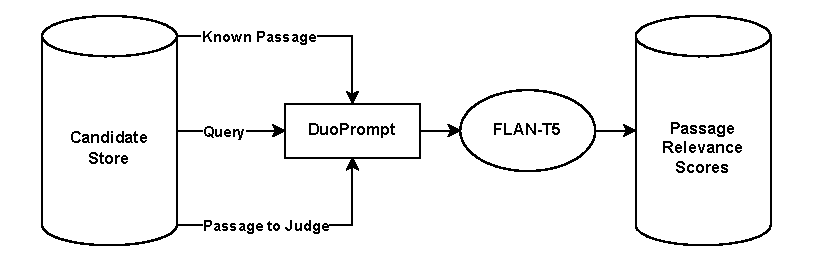
\includegraphics[width=\textwidth]{./graphics/drawio/pairwise_preferences.pdf}
    \caption{Visualization of the pairwise preference inference process with \texttt{DuoPrompt}. Each candidate consists of a query, a known passage from the source corpus, and a passage to judge from the target corpus.}
    \label{fig:pairwise-preferences}
\end{figure}

\begin{figure}[t]
    \centering
    \begin{tcolorbox}[title=DuoPrompt, width=\textwidth]
        \footnotesize
        \begin{verbatim}
PROMPT = (
    "Determine if passage B is as relevant as passage A "
    "for the given query. "
    'Passage A: "...{{ rel_doc_text | replace("\\"", "\'") }}..." '
    'Passage B: "...{{ unk_doc_text | replace("\\"", "\'") }}..." '
    'Query: "{{ query_text }}" '
    "Is passage B as relevant as passage A? </s>"
)
        \end{verbatim}
    \end{tcolorbox}
    \caption{One-shot \texttt{DuoPrompt} prompt instructing the model in Figure~\ref{fig:pairwise-preferences} to assess whether the passage to judge is as relevant as the known passage for a query.}
    \label{fig:oneshot-prompt}
\end{figure}

\noindent To perform the pairwise preference inference, the Python library \texttt{autoqrels}\footnote{\scriptsize https://github.com/seanmacavaney/autoqrels} was used. \texttt{autoqrels} is a tool designed for automatically inferring relevance judgments. It supports zero-shot and one-shot prompting for relevance inference and supports several pre-implemented inference models. The original \texttt{autoqrels} paper~\cite{macavaney:2023} evaluated the effectiveness of one-shot labelers for automatic relevance estimation. Among the tested approaches \texttt{MaxRep-BM25}, \texttt{MaxRep-TCT}, \texttt{DuoT5}, and \texttt{DuoPrompt}, the \texttt{DuoPrompt} approach for pairwise inference demonstrated superior performance and therefore is utilized for one-shot labeling in this thesis.
\\\\\\\\
Figure~\ref{fig:oneshot-prompt} illustrates the \texttt{DuoPrompt} structure used for pairwise inference with \texttt{FLAN-T5}. The prompt takes a query (\texttt{query\_text}), a known passage (\texttt{rel\_doc\_text}), and a passage to judge (\texttt{unk\_doc\_text}) as inputs. It includes a brief instruction for the model, asking it to compare the passage to judge with the known passage and assess its relevance to the query. The model then predicts a relevance score for the passage to judge. This structured comparison helps the model determine whether the passage to judge is as relevant as the known passage. If it is highly relevant, the expected score should be close to 1.0. Conversely, if it is not relevant at all, the \mbox{score should be close to 0.0}.
\\\\
\texttt{FLAN-T5} is a Text-to-Text Transfer Transformer model, an advanced version of Google's \texttt{T5} model~\cite{raffel:2020}. While maintaining the backbone architecture of \texttt{T5}, \texttt{FLAN-T5} has been further fine-tuned on a diverse set of training tasks, enhancing its performance across various natural language processing applications. \texttt{FLAN-T5} is available in multiple sizes, ranging from smaller, resource-efficient versions like \texttt{flan-t5-small}, with 80~million parameters, to models such as \texttt{flan-t5-xxl}, which contains 11~billion parameters. These variations accommodate different computational and application needs. Given the computational constraints for this thesis, \texttt{flan-t5-base}\footnote{\scriptsize https://huggingface.co/google/flan-t5-base} model, with 250 \mbox{million} parameters, is selected as the transformer model for \texttt{DuoPrompt}.
\\\\
All candidates undergo pairwise preference inference, where each passage to judged is compared against 20 known passages, as outlined in Section~\ref{composing-final-candidates}. As a result, the pairwise preference inference produces 20 relevance scores for each passage, with higher scores indicating greater relevance to the query. The overall relevance of each passage is then computed by aggregating its inferred scores, a process that will be detailed in the evaluation of Section~\ref{eval-pairwise-preferences}. To determine the final relevance score for a document, the maximum of all its passage scores is used. This approach follows the principle that a document's relevance is determined by its most relevant passage~\cite{craswell:2019}.
\\\\
This chapter provided a comprehensive description of all steps in the transfer pipeline, resulting in a set of relevance scores for each passage to judge. These scores represent the transferred information of the relevance judgments from a source dataset's retrieval task into a target document corpus. The next chapter will evaluate the effectiveness of the individual steps and the overall quality of the transferred relevance judgments across datasets.